% ****** Start of file apssamp.tex ******
%
%   This file is part of the APS files in the REVTeX 4 distribution.
%   Version 4.0 of REVTeX, August 2001
%
%   Copyright (c) 2001 The American Physical Society.
%
%   See the REVTeX 4 README file for restrictions and more information.
%
% TeX'ing this file requires that you have AMS-LaTeX 2.0 installed
% as well as the rest of the prerequisites for REVTeX 4.0
%
% See the REVTeX 4 README file
% It also requires running BibTeX. The commands are as follows:
%
%  1)  latex apssamp.tex
%  2)  bibtex apssamp
%  3)  latex apssamp.tex
%  4)  latex apssamp.tex
%
\documentclass[prb,aps,preprintnumbers,amsmath,amssymb]{revtex4}
%\documentclass[preprint,showpacs,preprintnumbers,amsmath,amssymb]{revtex4}

% Some other (several out of many) possibilities
%\documentclass[preprint,aps]{revtex4}
%\documentclass[preprint,aps,draft]{revtex4}
%\documentclass[prb,twocolumn,showpacs,preprintnumbers,amsmath,amssymb]{revtex4}% Physical Review B

\usepackage{graphicx}% Include figure files
\usepackage{dcolumn}% Align table columns on decimal point
\usepackage{bm}% bold math
\usepackage[utf8]{inputenc}
\usepackage{url}
\usepackage[spanish,es-tabla]{babel}
\newcommand{\nextitem}{\par\hspace*{\labelsep}\textbullet\hspace*{\labelsep}}
%\nofiles

\begin{document}

\title{Preinforme 3 - Amplificadores Operacionales}% Force line breaks with \\

\author{Alejandro Hernández A.}%
 \email{a.hernandez105@uniandes.edu.co}
\author{Jesús D. Prada G.}%
 \email{jd.prada1460@uniandes.edu.co}
\affiliation{%
Departamento de Física\\ Universidad de los Andes, Bogotá, Colombia.\\
}%

\date{16 de septiembre de 2015}% It is always \today, today,
             %  but any date may be explicitly specified

\begin{abstract}
En esta práctica de laboratorio se pretende aprender el funcionamiento experimental de amplificadores operacionales y mediante el uso de los mismos se pretende armar filtros activos y pasivos.\\

\noindent \textbf{Conceptos clave:} Amplificadores operacionales, filtros activos, filtros pasivos, ganancia.
\end{abstract}
                             
\maketitle

\section{Filtros activos y pasivos}
Como se ha mencionado en preinformes anteriores, un filtro es un sistema que permite el paso de señales eléctricas en un rango de
frecuencias determinadas e impide el paso del resto.\\

Un \textbf{filtro activo} se caracteriza por el uso de componentes activos. Dichos componentes se caracterizan por controlar el flujo de corriente en los circuitos o por realizar ganancias. Dichos elementos se enuncian a continuación \footnote{Información consultada en http://es.slideshare.net/electronicosdigitales/componentes-activos\\}.

\begin{itemize}
	\item \textbf{Amplificador operacional}: Como se puede apreciar en la figura \ref{fig: amplificador}, los amplificadores operacionales son dispositivos electrónicos con dos entradas y una salida, en la última de las cuales el potencial medido es la diferencia de potencial entre las dos entradas multiplicada por una constante $G$ que representa la ganancia de l sistema.
	
	\begin{figure}[h!]
		\centering
		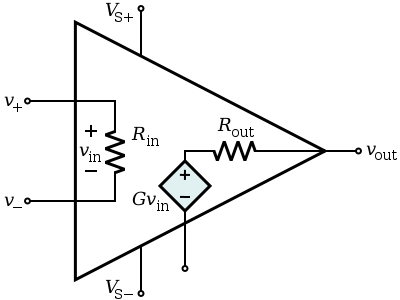
\includegraphics[width=0.5\textwidth]{amplificador}
		\caption{Amplificador operacional.}
		\label{fig: amplificador}
	\end{figure}
	
	\item \textbf{Diodos}: Típicamente utilizados para la rectificación y regulación de señales. 
	
	\item \textbf{Baterías}: Usadas para la generación de energía eléctrica.
	
	\item \textbf{Compuertas lógicas}: Empleadas para controlar el paso de la corriente eléctrica en un circuito de acuerdo con la función booleana asociada.
	
	\item \textbf{Transistor}: Usados para la amplificación o conmutación de señales.
\end{itemize}

Por su parte, los \textbf{filtros pasivos} se caracteriazan por usar componentes pasivos, en los cuales la potencia eléctrica absorbida es transformada en calor y que no son capaces de controlar el flujo de la corriente eléctrica. Estos componentes son los tres componentes típicos de cualquier circuito eléctrico, a saber\footnote{Información consultada en http://www.ecured.cu/index.php/Componentes\_electr\%C3\%B3nicos\_pasivos\\}: \\\\

\begin{itemize}
	\item \textbf{Resistencias}: Permiten controlar la corriente que pasa a través de un circuito.
		
	\item \textbf{Condensadores}: Sirven para almacenar energía en forma de carga eléctrica. 
	
	\item \textbf{Inductancias}: Se oponen al cambio del flujo de campo magnético a través de las mismas.
\end{itemize}

\begin{figure}
\centering
\begin{minipage}{.33\textwidth}
  \centering
  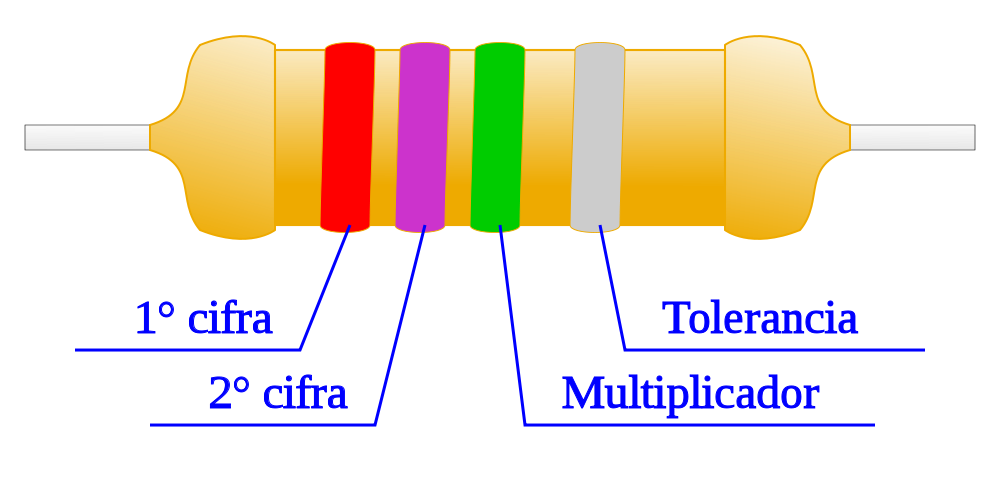
\includegraphics[width=.7\textwidth,height=0.15\textheight]{resistencia}
  \caption{Resistencia}
  \label{fig: resistencia}
\end{minipage}%
\begin{minipage}{.33\textwidth}
  \centering
  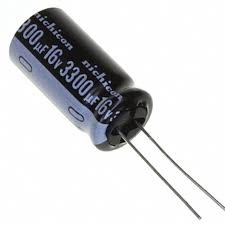
\includegraphics[width=.7\textwidth,height=0.15\textheight]{condensador}
  \caption{Condensador}
  \label{fig: condensador}
\end{minipage}
\begin{minipage}{.33\textwidth}
  \centering
  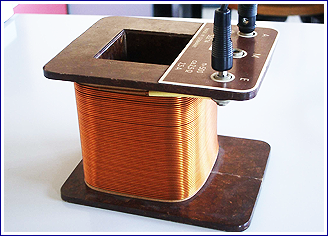
\includegraphics[width=.7\textwidth,height=0.15\textheight]{inductancia}
  \caption{Inductancia}
  \label{fig: inductancia}
\end{minipage}
\label{fig: pasivos}
\end{figure}

Las ventajas y desventajas de usar un filtro u otro se muestran a continuación \footnote{La información presentada se consultó en http://www.mty.itesm.mx/etie/deptos/ie/profesores/jgomez/eap/filtros.pdf\\}.\\

\textbf{Ventajas de los filtros activos}

\begin{itemize}
	\item Pueden ser usados sin inductancias, que son dispositivos electrónicos difíciles de conseguir, además de ser muy voluminosos para frecuencias bajas.
	
	\item Facilitan el montaje de filtros complejos mediante el ensamble de múltiples filtros simples.
	
	\item Proporcionan un gran ganancia, es decir, son buenos amplificadores de la señal de entrada, lo cual es especialmente útil.
	
	\item Se adaptan muy bien a las impedancias.
\end{itemize}

\textbf{Desventajas de los filtros activos}

\begin{itemize}
	\item Requieren de una fuente de alimentación externa para poder funcionar.
	
	\item Presentan una respuesta en freucuencia altamente limitada por la capacidad de los amplificadores operacionales usados.
	
	\item Es imposible implementar filtros activos en sistemas de media o alta potencia.
\end{itemize}

\textbf{Ventajas de los filtros pasivos}

\begin{itemize}
	\item Son económicos dado que sus componentes (salvo las inductancias) son de uso muy frecuente para el montaje de circuitos eléctricos básicos.
	
	\item Son fáciles de implementar.
	
	\item Su funcionamiento muestra una respuesta aproximada a la función ideal.
	
	\item Pueden ser usados en circuitos de altas frecuencias o altas potencias.
\end{itemize}

\textbf{Desventajas de los filtros pasivos}

\begin{itemize}
	\item La respuesta en frecuencia está limitada al valor de los componentes pasivos usados.
	
	\item Las inductancias no son fáciles de conseguir y su valor económico se incrementa para altas frecuencias.
\end{itemize}

Con respecto a las aplicaciones de dichos filtros, cabe mencionar que los filtros activos son frecuentemente usados en istrumentación y telecomunicaciones. En cuanto a la instrumentación, los dispositivos de bioelectrónica o electromedicina típicamente incluyen este tipo de filtros puesto que necesitan trabajar con señales de bajas frecuencias. \\

Los filtros tanto activos como pasivos también se usan para aumentar o atenuar frecuencias en circuitos de audio, generadores electrónicos de música, instrumentos sísmicos y circuitos de comunicaciones. Además, en ámbitos experimentales o de laboatorio, son utilizados para estudiar señales de ondas cerebrales y vibraciones mecánicas.\\

\section{Tipos de filtros ativos}


\begin{thebibliography}{99}
\
\\
\bibitem{resistencia} La imagen de la resistencia se obtuvo en http://www.areatecnologia.com/electricidad/resistencia-electrica.html.\\

\bibitem{condensador} La imagen del condensador se obtuvo en http://logicadigitaltemario2.blogspot.com.co/2015/04/condensador.html.\\

\bibitem{inductancia} La imagen de la inductancia se obtuvo en http://www.electricaindustrialmaldonado.com/fabricacion-de-bobinas.\\


\end{thebibliography}

\end{document}
%
% ****** End of file apssamp.tex ******
